
\newpage
\section{Conclusion}\label{sec:6}

Overall, there is no singular optimal method for explaining models or constructing interpretable ones. While XAI has gained significant attention, it is crucial to acknowledge the inherent limitations of each approach and refrain from using them blindly. When used properly, XAI can yield substantial advantages. However, it remains an area of active research.

In conclusion, I would like to provide four key takeaways that I have learned from my study.

\subsubsection*{1. The selection of the XAI approach is goal and risk-specific.}
In Section \ref{sec:goals}, we discussed the various goals associated with XAI. Different XAI approaches may be favored depending on the specific goal pursued. \\
Additionally, the choice of an approach depends on the context in which ML is applied and the particular task at hand. For instance, in environments where there are high risks involved and critical decisions must be made, it is advisable to use inherently interpretable models, as suggested by \cite{rudin2019stop}.

\subsubsection*{2. For the same model different explanations for different people.}
As mentioned in Subsection \ref{sec:goals}, the audience you're addressing significantly influences the approach you should take in providing explanations. Certain techniques may not be appropriate for individuals with limited knowledge of ML. On the other hand, more complex approaches can be used for experts in the field.

\subsubsection*{3. Many XAI methods have problems with correlated features.}
As observed in techniques such as Linear Regression or Permutation Feature Importance, various methods are sensitive to the presence of correlated features, which can greatly affect the result of the explanations provided.
To address this issue, one can use feature engineering techniques to reduce feature correlation before training. This can involve either introducing new features or excluding highly correlated ones.

\subsubsection*{4. No linear relationship between accuracy and interpretability.}
Some people may believe that highly complex models offer the best accuracy, assuming that a complex "black box" approach is essential for achieving top predictive performance. However, according to \cite{rudin2019stop}, this isn't always the case, especially when dealing with well-structured data containing naturally meaningful features, there's often no notable difference in performance between complex models like deep neural networks and much simpler ones like logistic regression. Figure \ref{fig:tradeoff} displays the misconception:

\begin{figure}[H]
    \centering
    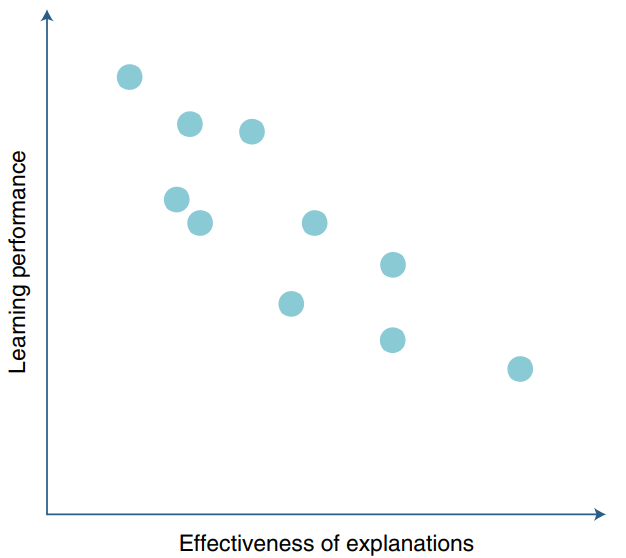
\includegraphics[width=0.5\linewidth]{pics/fictional_depiction.png}
    \caption[A fictional depiction of the accuracy–interpretability trade-off.]{A fictional depiction of the accuracy–interpretability trade-off.\cite{rudin2019stop}}
    \label{fig:tradeoff}
\end{figure}
